\documentclass[11pt,a4paper]{article}
\usepackage[utf8]{inputenc}
\usepackage{amsmath}
\usepackage{amsfonts}
\usepackage{graphicx}
\usepackage[table,xcdraw]{xcolor}

\DeclareUnicodeCharacter{00A0}{ } %este rollo es para evitar un error por la aparición de un caracter invisible e hijo de puta

\usepackage{caption}
\usepackage{subcaption}

\renewcommand{\familydefault}{\sfdefault} % cambiamos la fuente a una sans

\usepackage{float} % para que floten las imagenes o algo asi...
\usepackage{wallpaper} %paquete para usar una imagen como encabezado!
\usepackage{hyperref} %para usar hypervinculos 
\usepackage[export]{adjustbox} %para usar marcos en imagenes
\usepackage{eurosym} % para el euro
\usepackage{transparent} %para las marcas de agua
\usepackage{eso-pic}  %para las marcas de agua

\definecolor{azul_marcos}{RGB}{0,128,159} %defino el color azul de los marcos
\usepackage{sectsty} %esto es para cambiar el color de las fuentes creo
\renewcommand{\familydefault}{\sfdefault} % cambiamos la fuente a una sans
\sectionfont{\color{azul_marcos}}  % sets colour of sections
\subsectionfont{\color{azul_marcos}}  % sets colour of sections


\usepackage{pdfpages} %para insertar pdfs
\usepackage{amssymb}
\usepackage{pstcol} % para color
\usepackage{pst-node} % para diagramas
\usepackage{pst-plot} % para representacion de dat
\usepackage[spanish]{babel}
\addto\captionsspanish{\renewcommand\chaptername{Bloque}}
%\usepackage[total={18cm,21cm},top=2cm, left=2cm]{geometry}
\usepackage{anysize}
\pagestyle{plain}
%\markboth{left head}{right head}
%\markright{Guía de impresión ABS Tech}
\marginsize{3cm}{2cm}{2.5cm}{1cm}
\title{Guía de impresión ABS Tech}
\date{}

%configuracion de la marca de agua
\AddToShipoutPicture{
    \put(0,0){
        \parbox[b][\paperheight]{\paperwidth}{%
            \vfill
            \centering
            {\transparent{0.1}
\includegraphics[scale=1.25]{FOTOS/logofff}}%
            \vfill
        }
    }
}

\begin{document}
\ULCornerWallPaper{1}{FOTOS/header}
\LLCornerWallPaper{1}{FOTOS/footer}
%\maketitle
%\tableofcontents

\includepdf{PDF/PORTADA.pdf}
\section{¿Qué es el filamento PETG Tech?}PETG Tech es un filamento para impresión 3D FFF/FDM de tereftalato de polietileno glycol (P.E.T.G.) diseñado para combinar lo mejor del PLA y del ABS siendo un termoplástico resistente y fácil de imprimir.
\begin{figure}[H]
\centering
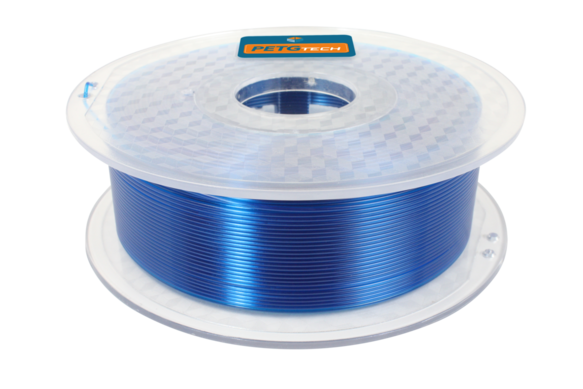
\includegraphics[width=0.5\textwidth,cfbox=azul_marcos 1pt 0pt]{FOTOS/PETGKILOAZUL}
\end{figure}
\section{¿Por qué usar filamento 3D PETG Tech?}
PETG Tech es uno de los filamentos más versátiles del mercado ya que combina las mejores propiedades de otros materiales.
\begin{itemize}
\item El PETG es muy resistente, casi tanto como el ABS, así que puede ser utilizado para construir piezas que vayan a sufrir stress mecánico por tracción, presión o impacto.
\item El PETG también soporta mejor la temperatura que el PLA y tiene una buena resistencia ante químicos y disolventes. También resiste mejor la exposición a rayos UV que el PLA y el ABS.
\item Al ser una material poco higroscópico se conserva mejor y más fácilmente que el PLA.
\item Además el PETG presenta mucho menos “warping” (o tendencia a deformarse al enfriarse) que el ABS y, con los métodos adecuados, éste puede ser controlado completamente. Por ello el PETG, a diferencia  permite la impresión de volúmenes grandes en impresoras domésticas.
\item Aunque el filamento de PETG no tiene certificación para estar en contacto con alimentos (FDA Food Safety) el pellet a partir del cual se fabrica sí que la tiene y esto hace que sea más indicado para un eventual contacto con alimentos que el resto de materiales. Más adelante analizamos a fondo este aspecto.
\item El PETG es un material reciclable y biodegradable al igual que PLA.
\item El PETG es naturalmente translucido y brillante. Aunque también se vende en colores opacos estos conservan un acabado brillante.
\end{itemize}

A continuación presentamos una tabla comparativa entre el PETG el PLA y el ABS:
\begin{table}[H]
\centering
\begin{tabular}{l|c|c|c|}
\cline{2-4}
                                                                                      & \cellcolor[HTML]{FFFFFF}PLA & \cellcolor[HTML]{FFFFFF}ABS & \cellcolor[HTML]{FFFFFF}PETG \\ \hline
\rowcolor[HTML]{FFFFFF} 
\multicolumn{1}{|l|}{\cellcolor[HTML]{FFFFFF}Elevada resistencia al impacto}          &                             & X                           & X                            \\ \hline
\rowcolor[HTML]{FFFFFF} 
\multicolumn{1}{|l|}{\cellcolor[HTML]{FFFFFF}Baja deformación al enfriarse (warping)} & X                           &                             & X                            \\ \hline
\rowcolor[HTML]{FFFFFF} 
\multicolumn{1}{|l|}{\cellcolor[HTML]{FFFFFF}Absorbe poca humedad}                    &                             & X                           & X                            \\ \hline
\rowcolor[HTML]{FFFFFF} 
\multicolumn{1}{|l|}{\cellcolor[HTML]{FFFFFF}Biodegradable}                           & X                           &                             & X                            \\ \hline
\rowcolor[HTML]{FFFFFF} 
\multicolumn{1}{|l|}{\cellcolor[HTML]{FFFFFF}FDA Food safety *}                       &                             &                             & X                            \\ \hline
\rowcolor[HTML]{FFFFFF} 
\multicolumn{1}{|l|}{\cellcolor[HTML]{FFFFFF}Buena resistencia a rayos UV}            &                             &                             & X                            \\ \hline
\rowcolor[HTML]{FFFFFF} 
\multicolumn{1}{|l|}{\cellcolor[HTML]{FFFFFF}Sin olor al ser impreso}                 & X                           &                             & X                            \\ \hline
\end{tabular}
\end{table}
\section{Ficha técnica y parámetros de impresión}
\begin{table}[H]
\centering
\caption*{Ficha técnica}
\begin{tabular}{|
>{\columncolor[HTML]{FFFFFF}}l |
>{\columncolor[HTML]{FFFFFF}}c |}
\hline
\multicolumn{1}{|c|}{\cellcolor[HTML]{FFFFFF}\textbf{Material}}   & Tereftalato de polietileno glycol   \\ \hline
\textbf{Colores disponibles}              & 5 (3 translucidos, 2 opacos)                 \\ \hline
\textbf{Formatos disponibles}             & 1kg, 250gr         \\ \hline
\textbf{Temperatura de deflexión térmica} & 70               \\ \hline
\textbf{Temperatura de fusión}            & 200ºC              \\ \hline
\textbf{Temperatura de descomposición}    & \textgreater 280ºC \\ \hline
\textbf{Densidad}                         & 1.27 gr / cm3      \\ \hline
\textbf{Resistencia al impacto}                         & 100 kg-cm / cm      \\ \hline
\textbf{Estiramiento máximo}              & 140\%              \\ \hline
\end{tabular}
\end{table}

%TABLA PARAMETROS IMPRESION MEDIA

\begin{table}[H]
\centering
\caption*{Parámetros de impresión medios recomendados}
\begin{tabular}{|
>{\columncolor[HTML]{FFFFFF}}l |
>{\columncolor[HTML]{FFFFFF}}c |}
\hline
\multicolumn{1}{|c|}{\cellcolor[HTML]{FFFFFF}\textbf{Temperatura recomendada de impresión}} & 245º              \\ \hline
\textbf{Velocidad recomendada de impresión}                         & 55 mm/s              \\ \hline
\textbf{Altura de capa}                                  &  0.2 mm        \\ \hline
\textbf{Temperatura cama caliente}                                  &  70º - 85º        \\ \hline
\textbf{Ventilador de capa}                                  &  75\%        \\ \hline
\textbf{Extrusion multiplier **}                                  &  85\% / 100\%        \\ \hline

\textbf{Retracción ***}                                      & Normal o aumentada                 \\ \hline
\end{tabular}
\end{table}

%TABLA PARAMETROS RESISTENCIA

\begin{table}[H]
\centering
\caption*{Parámetros de impresión recomendados para máxima resistencia y menor transparencia *}
\begin{tabular}{|
>{\columncolor[HTML]{FFFFFF}}l |
>{\columncolor[HTML]{FFFFFF}}c |}
\hline
\multicolumn{1}{|c|}{\cellcolor[HTML]{FFFFFF}\textbf{Temperatura recomendada de impresión}} & 260º              \\ \hline
\textbf{Velocidad recomendada de impresión}                         & 40 mm/s              \\ \hline
\textbf{Altura de capa}                                  &  0.2 mm        \\ \hline
\textbf{Temperatura cama caliente}                                  &  70º - 85º        \\ \hline
\textbf{Ventilador de capa}                                  &  Desactivado       \\ \hline
\textbf{Extrusion multiplier **}                                  &  85\% / 100\%        \\ \hline

\textbf{Retracción ***}                                      & Normal o aumentada                 \\ \hline
\end{tabular}
\end{table}

%TABLA PARAMETROS TRANSPARENCIA

\begin{table}[H]
\centering
\caption*{Parámetros de impresión recomendados para máxima transparencia * y menor resistencia}
\begin{tabular}{|
>{\columncolor[HTML]{FFFFFF}}l |
>{\columncolor[HTML]{FFFFFF}}c |}
\hline
\multicolumn{1}{|c|}{\cellcolor[HTML]{FFFFFF}\textbf{Temperatura recomendada de impresión}} & 235º - 240º              \\ \hline
\textbf{Velocidad recomendada de impresión}                         & 70 mm/s              \\ \hline
\textbf{Altura de capa}                                  &  0.3 mm        \\ \hline
\textbf{Número de perímetros}                                  &  1        \\ \hline
\textbf{Infill}                                  &  0\%        \\ \hline
\textbf{Temperatura cama caliente}                                  &  70º - 85º        \\ \hline
\textbf{Ventilador de capa}                                  &  100\%        \\ \hline
\textbf{Extrusion multiplier **}                                  &  85\% / 100\%        \\ \hline

\textbf{Retracción ***}                                      & Normal o aumentada                 \\ \hline
\end{tabular}
\end{table}

* Sólo pueden esperarse acabados cristalinos en piezas huecas con un solo perímetro, idealmente objetos de tipo vaso.

** En algunas impresoras puede ser necesario reducir el extrusión multiplier. Si observa un exceso de material en la pieza impresa en forma de pequeñas bolas de plástico o nota que el nozzle choca con la pieza durante la impresión, reduzca el extrusión multiplier al 85\% y auméntelo progresivamente hasta encontrar el punto en el que la extrusión sea la adecuada.

*** Si tiene problemas de stringing pruebe a aumentar la velocidad y la distancia de retracción.
\\\\
Puedes descargarte nuestros perfiles completos de impresión de los principales programas de laminación (Cura, Slic3r y Simplify3D) desde nuestra página web:
\\\\
\centerline{ {\huge \url{www.fffworld.com/documentation} } }
\\\\
Los parámetros óptimos dependerán de la impresora 3D que utilices, sin embargo, son unos buenos parámetros para tenerlos como punto de partida. Con unas pocas impresiones serás capaz de encontrar los límites y la configuración perfecta para tu maquina.
\section{PETG Tech: Características y consejos de impresión}
	\subsection{La resistencia del PETG}PETG Tech puede ser utilizado para fabricar piezas extraordinariamente resistentes.
\\\\
El PETG es ligeramente flexible y esto le permite absorber energía antes de romperse pero lo que realmente marca la diferencia con otros materiales es la consistencia de la unión entre capas que este material proporciona.
\begin{figure}[H]
\centering
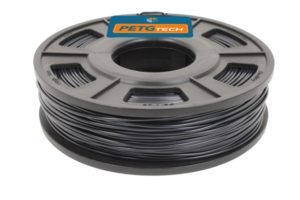
\includegraphics[width=0.5\textwidth,cfbox=azul_marcos 1pt 0pt]{FOTOS/PETG250NEGRO}
\end{figure}
La adherencia de las capas es tan firme que en ocasiones las piezas tienen mayor resistencia a la tracción entre capas que en el eje longitudinal a la pista de filamento extruido.
\\\\La resistencia entre capas puede aumentarse elevando la temperatura o disminuyendo la velocidad. Esto permite que el material derretido se deposite más caliente y más despacio. Sin embargo el acabado de la pieza será peor y la transparencia se reducirá como consecuencia de pistas de plástico ligeramente deformadas por el exceso de temperatura.
\\\\El ventilador de capa aquí juega a favor de la transparencia y del acabado y en contra de la resistencia general de la pieza. No obstante los programas de laminado actuales permiten activarlo durante momentos concretos de la impresión.
\\\\Tenga en cuenta lo anterior a la hora de laminar, dependiendo del tipo de pieza y el uso que le vaya a dar.
	\subsection{La transparencia del PETG}El PETG es un material translúcido al igual que el PET que se utiliza en la fabricación de envases plásticos totalmente transparentes.
\begin{figure}[H]
\centering
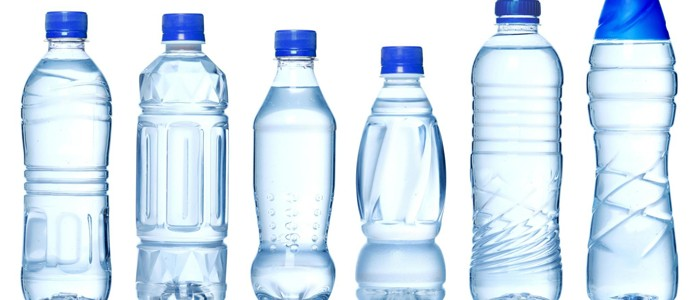
\includegraphics[width=0.5\textwidth,cfbox=azul_marcos 1pt 0pt]{FOTOS/BOTELLASPET}
\end{figure}
No obstante hay que tener en cuenta que los procesos de fabricación de dichos envases difieren enormemente de los utilizados en impresión 3D  y por ello conseguir pieza impresas en 3D completamente cristalinas no es posible, al menos usando tecnología FFF/FDM.
\\\\
Esto es provocado por irregularidades especulares que se crean en el interior de la pieza como consecuencia del proceso de deposición de capas de plástico.
\\\\
Además al acumular perímetros horizontales el incremento del grosor de las paredes de las piezas reduce la transparencia.
\\\\
No obstante si su objetivo es conseguir piezas translúcidas le proponemos algunos trucos.
\\\\
Como norma general cuanto mayor es la temperatura o más baja es la velocidad, la transparencia de la pieza impresa es menor. Esto es debido a que el plástico caliente tiende a escurrir creando superficies curvas que desvían la luz.
\\\\
Con velocidades más altas y temperaturas más bajas se puede conseguir que las pistas de plástico fundido queden depositadas de manera más regular favoreciendo la transparencia de la pieza.
\\\\
Dependiendo del eje en el que necesite un acabado más translúcido puede seguir también los siguientes consejos:
		\subsubsection{Transparencia en eje Z (vertical)}La transparencia de la pieza va a ser función de la altura de la misma y del infill utilizado.
\\\\
También del número de capas así que la recomendación es utilizar una altura de capa mayor para reducir el número de las mismas.
\\\\
Hay que diferenciar entre las capas que componen la base de la pieza, y que se imprimen directamente sobre la superficie de impresión, de aquellas que sirven de tapa o cerramiento superior.
\\\\
En las primeras la transparencia será buena puesto que el plástico fundido toma una forma plana y regular al ser depositado en una superficie plana.
\\\\
Las superiores sin embargo tienden a arquearse puesto que quedan apoyadas sobre los perímetros horizontales exteriores y la estructura de relleno.
\\\\
Por ello las capas inferiores tienen mejor transparencia que las superiores.
\\\\
Para atenuar este problema puede aumentar la velocidad con la que la impresora extruye las capas superiores de forma que éstas queden más tensas y menos irregulares. Esta es una opción avanzada que no está disponible en todos los programas de laminado.
		\subsubsection{Transparencia en plano XY (horizontal)}En el plano XY la forma de aumentar la transparencia es reducir el número de perímetros.
\\\\
No obstante si la pieza tiene algún tipo de infill éste va a restar transparencia igualmente así que sólo es posible conseguir piezas con alta transparencia en piezas de tipo vaso.
\\\\
Para este tipo de piezas los programas de laminado ofrecen la opción de imprimir aumentando la posición Z de manera continua cuando se quiere imprimir con un solo perímetro. Esta opción se conoce como spiralize (Cura), o vase mode (Slic3r y Simplify) y es la que recomendamos en orden a obtener los mejores resultados en cuanto a transparencia.
\\\\
Como ya hemos comentado cuanto mayor sea la velocidad y menor la temperatura mejor será la transparencia como consecuencia de una disposición más regular y tensa de las pistas de plástico así que las pruebas deberán ir encaminadas a encontrar la velocidad máxima y la temperatura mínima que permita imprimir piezas sin que las capas se separen.
\\\\
Una velocidad de 70 mm\/s con una temperatura de 240º y una altura de capa de 0.25 mm debería proporcionar una buena transparencia en piezas impresas en modo vaso (vase mode) aunque esto es dependiente de la pieza y de la máquina.
	\subsection{El filamento 3D PETG y la seguridad alimentaria (FDA Food Safety) de los objetos impresos en 3D}El PETG y el PET son plásticos muy similares y es sabido que este último se utiliza de manera generalizada en la fabricación de envases plásticos contenedores de alimentos. Es así porque ambos cuentan con una certificación expedida por la FDA que garantiza la salubridad de alimentos que entren en contacto con dichos materiales.
\begin{figure}[H]
\centering
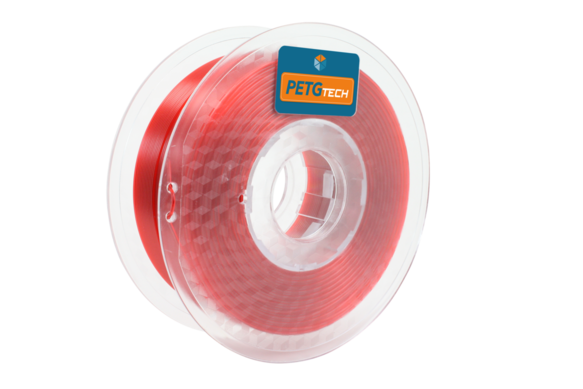
\includegraphics[width=0.5\textwidth,cfbox=azul_marcos 1pt 0pt]{FOTOS/PETGKILOROJO}
\end{figure}
Si bien esto es cierto hay que entender que dicha certificación se refiere al pellet (materia prima) a partir del cual se fabrican los filamentos de PETG y que dicha certificación no puede transponerse directamente por diferentes motivos que vamos a analizar.
\\\\
En primer lugar los filamentos para impresión 3D suelen contener aditivos para dotarlos de características que mejoren su rendimiento al ser utilizados. La inclusión de cualquier aditivo que no tenga certificación FDA Food Safety impide que ésta se aplique.
\\\\
Por otra parte la mayoría de los filamentos son mezclados con tintes para dotarlos de color y aunque estos tintes cuentan con certificación ROHS no cuentan con certificación FDA Food Safety.
\\\\
La primera (ROHS) certifica la ausencia de elementos manifiestamente nocivos (como el plomo o el mercurio) mientras que la segunda certifica la absoluta inocuidad del objeto certificado hasta el punto de que puede estar en contacto durante largo tiempo con alimentos destinados al consumo. Por lo tanto la mera adición de tintes no FDA Food Safety impiden su consideración como tal.
\begin{figure}[H]
\centering
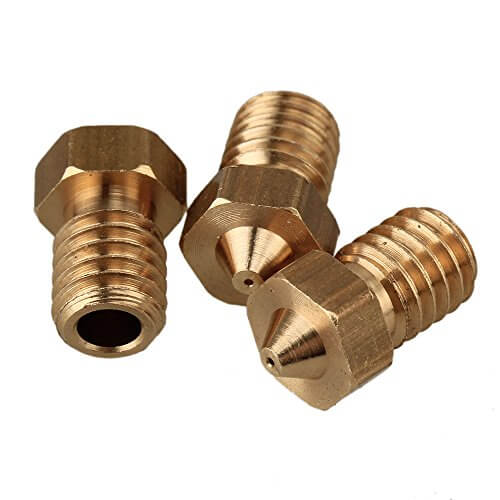
\includegraphics[width=0.5\textwidth,cfbox=azul_marcos 1pt 0pt]{FOTOS/NOZZLES}
\caption*{Los nozzles pueden contener plomo}
\end{figure}
Incluso en el supuesto de filamentos cuyo material base, aditivos y tintes cuenten con certificación FDA Food Safety el proceso de impresión en una máquina doméstica impide que el objeto resultante pueda certificarse. Esto como consecuencia de los metales con los que se fabrica el nozzle (latón) y del extrusor que empuja el filamento.
\\\\
Por todo lo anterior no es posible crear objetos mediante impresión 3D FFF que cumplan con la normativa FDA Food Safety
\\\\
Con todo lo anterior es necesario establecer la diferencia entre seguridad alimentaria especial y general.
\\\\
La primera es la que otorgan agencias como la FDA, garantiza la salubridad y están obligadas a ofrecer determinadas empresas en sus productos.
\\\\
La segunda, la seguridad alimentaria general, es la confianza que cualquiera puede tener, en base a su razón y experiencia, en que un determinado alimento no contiene ningún elemento manifiestamente nocivo tras su manipulación.
\\\\
Si bien los objetos impresos en 3D no pueden tener certificación FDA es seguro suponer que nadie pueda intoxicarse por comer una galleta que haya sido cortada con un molde de galletas impreso en 3D o utilizando un vaso o un cubierto desechable impreso en 3D.
\begin{figure}[H]
\centering
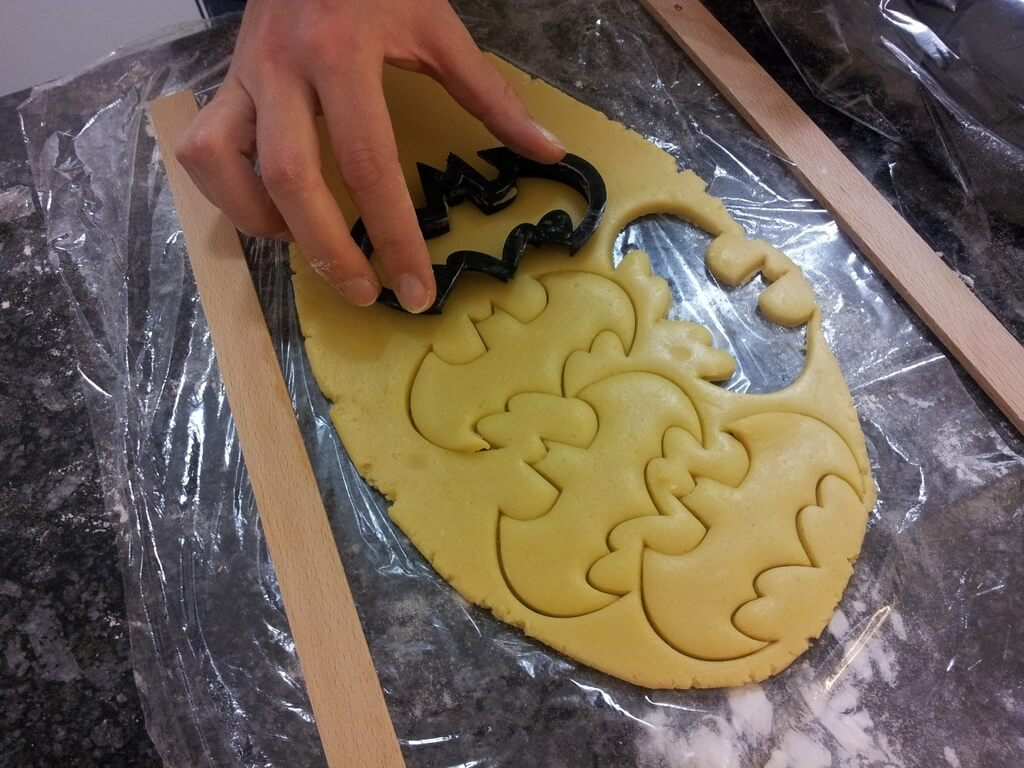
\includegraphics[width=0.5\textwidth,cfbox=azul_marcos 1pt 0pt]{FOTOS/CORTADORGALLETAS}
\end{figure}
Ahora bien hay que tener en cuenta algunas cosas a la hora de imprimir objetos que vayan a estar en contacto con alimentos:
\\\\
La impresión 3D FFF/FDM tiende a dejar pequeños espacios e intersticios en la superficie de las piezas que favorecen el desarrollo de bacterias y microorganismos. Si la pieza va ser de un solo uso puede no ser un problema pero si va a reutilizarse considere la posibilidad de aplicar un recubrimiento epoxi Food Safety para sellar la superficie de la pieza. 
\\\\
Dichos organismos deberían morir al utilizar un lavavajillas por la elevada temperatura del agua pero dicha temperatura puede deformar la pieza.
\\\\
El tiempo de contacto entre el alimento y la pieza es importante; no es lo mismo una botella que un tenedor o un cortador de galletas.
\section{Problemas y soluciones al imprimir filamento 3D PETG}
	\subsection{Cómo adherir correctamente el PETG a la superficie de impresión}El PETG tiene menos warping que el ABS y puede ser controlado, no obstante es necesario que la primera capa quede perfectamente pegada a la superficie de impresión en orden a imprimir satisfactoriamente.
\\\\
El mejor método es utilizar cama caliente a 75º e imprimir sobre el cristal aplicando laca standard.
\\\\
En caso de no disponer de cama caliente se recomienda utilizar la opción brim del programa de laminado y bajar la velocidad de la primera capa de forma que ésta quede firmemente adherida a la superficie de impresión.
\begin{figure}[H]
\centering
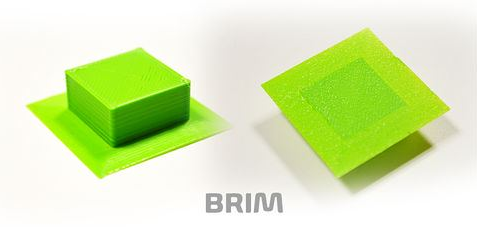
\includegraphics[width=0.5\textwidth,cfbox=azul_marcos 1pt 0pt]{FOTOS/BRIM}
\end{figure}
Se han observado problemas a tratar de imprimir filamento 3D PETG sobre cinta azul (3M blue tape) o cinta de carrocero por lo que recomendamos utilizar el primer método descrito: laca, cristal y cama a a 75º
	\subsection{Las estructuras de soporte en PETG}Ya hemos hablado de lo fuerte que es la unión entre las capas de PETG fundido, sin embargo esto presenta un reto a la hora imprimir piezas que hagan uso intensivo de estructuras de soporte.
\\\\
Ya hemos hablado de lo fuerte que es la unión entre las capas de PETG fundido, sin embargo esto presenta un reto a la hora imprimir piezas que hagan uso intensivo de estructuras de soporte.
\\\\
Los soportes de PETG se retiran con mayor dificultad y el acabado de la superficie en contacto directo con el soporte es áspero e irregular.
\\\\
Los programas de laminado más avanzados permiten configurar la distancia horizontal y vertical  entre la pieza y los soportes, así como el infill y la geometría de la estructura de soporte.
\\\\
Se recomienda aumentar dichas distancias, reducir el infill del soporte y optar por una geometría simple de lineas si está teniendo alguno de los problemas mencionados al utilizar estructuras de soporte en sus piezas.
	\subsection{Problemas de stringing}La capacidad del PETG para pegarse fuertemente lo hace propenso a dejar restos en forma de hilos en las piezas impresas.
\begin{figure}[H]
\centering
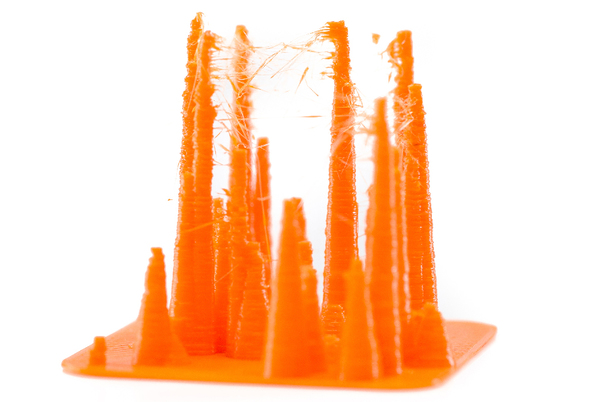
\includegraphics[width=0.5\textwidth,cfbox=azul_marcos 1pt 0pt]{FOTOS/RETRACCION1}
\caption*{Pieza con problemas de stringing}
\end{figure}
Como ya hemos comentado anteriormente este efecto puede reducirse haciendo uso de la retracción, pero es muy recomendable que además las distintas piezas se impriman de manera secuencial en vez de simultánea.
\\\\
Con impresión secuencial nos referimos a imprimir completamente una pieza antes de empezar a imprimir la siguiente.
\\\\
Esto se puede conseguir de 2 maneras diferentes:
\begin{itemize}
\item La opción trivial es imprimir sólo una pieza y una vez terminada repetir la misma impresión tantas veces como se quiera.
\item La segunda alternativa, más avanzada y con algunas limitaciones, es hacer uso de la opción que ofrecen algunos programas de laminado de imprimir una pieza cada vez. El tamaño máximo de las piezas que pueden ser impresas usando este método viene dado por las dimensiones del nozzle y la disposición de los ejes de la impresora. Recomendamos encarecidamente que te informes acerca de cómo usar estas opciones para no correr riesgo de dañar tu impresora. Puedes hacerlo a través de los siguientes enlaces:
\end{itemize}
\url{https://www.simplify3d.com/support/tutorials/multi-part-printing/}\\
\url{http://manual.slic3r.org/advanced/sequential-printing}\\
\url{https://ultimaker.com/en/community/3843-force-cura-to-print-objects-separately}
\begin{figure}[H]
\centering
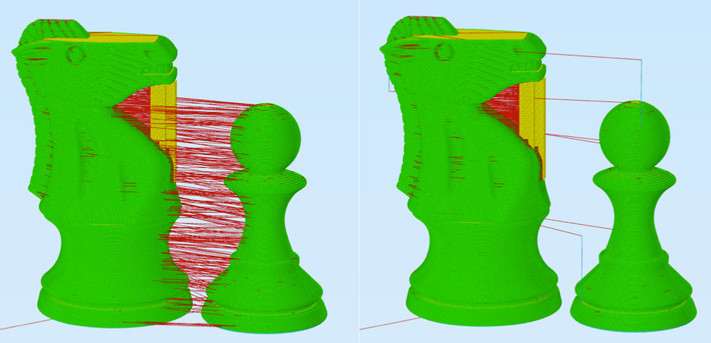
\includegraphics[width=0.5\textwidth,cfbox=azul_marcos 4pt 0pt]{FOTOS/SEQUENTIALPRINTING}
\caption*{Comparación de las rutas de impresión entre impresion simultanea y secuencial}
\end{figure}
\section{¿Quieres apoyar nuestro proyecto?}
Todos los miembros FFF World amamos la impresión 3D y la comunidad maker. Nos sentimos afortunados de poder trabajar en proyectos donde podamos entregar nuestra pasión sincera. En el futuro, nos gustaría poder desarrollar más materiales, más colores, más formatos. En definitiva, nos gustaría poder hacer crecer nuestra empresa.
\\\\
Para ello, una de las principales acciones para ayudarnos, si quieres hacerlo y estás satisfecho con el filamento, es la de votarnos en Amazon con 5 estrellas.
\begin{figure}[H]
\centering

\includegraphics[width=0.5\textwidth,cfbox=azul_marcos 1pt 0pt]{FOTOS/AMAZON_FIVE_STARS}
\caption*{¡Muchas gracias!}
\end{figure}
\subsection{Otros materiales con propiedades fantásticas disponibles en Amazon}
\begin{description}
\item[FlexiSMART Tech:] Diseñado para resistir a la abrasión y al desgaste de impresiones técnicas.
\item[ABS Tech:] Efecto warping minimizado. Alto rendimiento en aplicaciones técnicas.
\item[PETG Tech:] Máxima resistencia mécanica. Resistente al contacto con el agua y los rayos UV. Apto para uso alimentario.
\item[FilaMETAL:] PLA con carga metálica no abrasiva que da un acabado metálico espectacular a tus impresiones.
\item[PC Tech:] Policarbonato con gran resistencia a la temperatura y con excelentes propiedades mecánicas.
\item[Nylon Tech:] Imprimible a baja temperatura. Resistencia a los golpes con cierto grado de flexibilidad.
\item[PVA Tech:] Filamento soluble en agua indicado para uso como material de soporte. Excelente compatibilidad con PLA.
\item[HIPS Tech:] Filamento soluble en limoneno indicado para uso como material de soporte. Buena resistencia mecánica y excelente compatibilidad con ABS.
\end{description}
%\section{Bibliografía}
%Esta guía no habría sido posible sin el conocimiento libre generado por la comunidad RepRap. Para la elaboración de esta guía se han %utilizado imágenes y contenido extraidos de los siguientes sitios web.
%\\\\
%\url{http://www.gyrobot.co.uk/blog/how-to-3d-print-with-flexible-filaments}\\
%\url{http://www.thingiverse.com/thing:1496895}\\
%\url{http://www.thingiverse.com/thing:247024}\\
%\url{http://www.thingiverse.com/thing:16319}\\
%\url{http://www.thingiverse.com/thing:779011}\\
%\url{http://www.thingiverse.com/thing:1102900}\\
%\url{http://www.thingiverse.com/thing:147705}\\
%\url{http://www.thingiverse.com/thing:222667}\\
%\url{http://www.thingiverse.com/thing:512338}\\
%\url{https://all3dp.com/common-3d-printing-problems-and-their-solutions/}\\
%\url{https://www.simplify3d.com/support/}\\
%\url{http://www.thingiverse.com/thing:508896}\\
%\url{http://www.thingiverse.com/thing:1187344}

\includepdf{PDF/ES_CONTRAPORTADA.pdf}
\end{document}
